\section{\label{sec:paraview}Paraview}

For this part of the tutorial we are going to use Paraview, an easy to use, open source visualization program for scientific data. You should find a preinstalled version on the CIP pool computers, which you can execute with the command
%
\begin{center}
\texttt{paraview}
\end{center}
%
If you want to use it on other computers, it is part of most Linux distributions' repositories or you can get a copy at \href{http://www.paraview.org/}{http://www.paraview.org/}.

You can output the LB velocity field and the boundary geometry from \ES{} in a Paraview compatible format with the following commands
%
\begin{itemize}
\item \texttt{lbfluid print vtk boundary \textit{filename}}
\item \texttt{lbfluid print vtk velocity \textit{filename}}
\end{itemize}
%
while the particle coordinates can be output using
\begin{itemize}
\item \texttt{writevtk \textit{filename} [\textit{particle-type}]}
\end{itemize}
%
If no particle type id is given, all particle coordinates are written.

Filenames should always carry the suffix \texttt{.vtk}, so that Paraview automatically selects the correct reader upon opening. If you want to create a time series (video), you should name your files \texttt{filename\_CTR.vtk} with CTR a number incremented for every frame. You can then load all these files at one with Paraview and use the video controls to step through time.

Paraview is a very flexible visualization program. You can use the GUI to create very specific visualizations for your data. Visualization methods and data post processing algorithms are contained in so-called \textit{filters}. Filters can be chained and filter chains form a \textit{pipeline} which can be manipulated using the \textit{pipeline-browser}. For a start, it will be sufficient to know about the 7 Paraview controls shown in Figure~\ref{fig:paraview}.
%
\begin{figure}[htp]
\begin{center}
  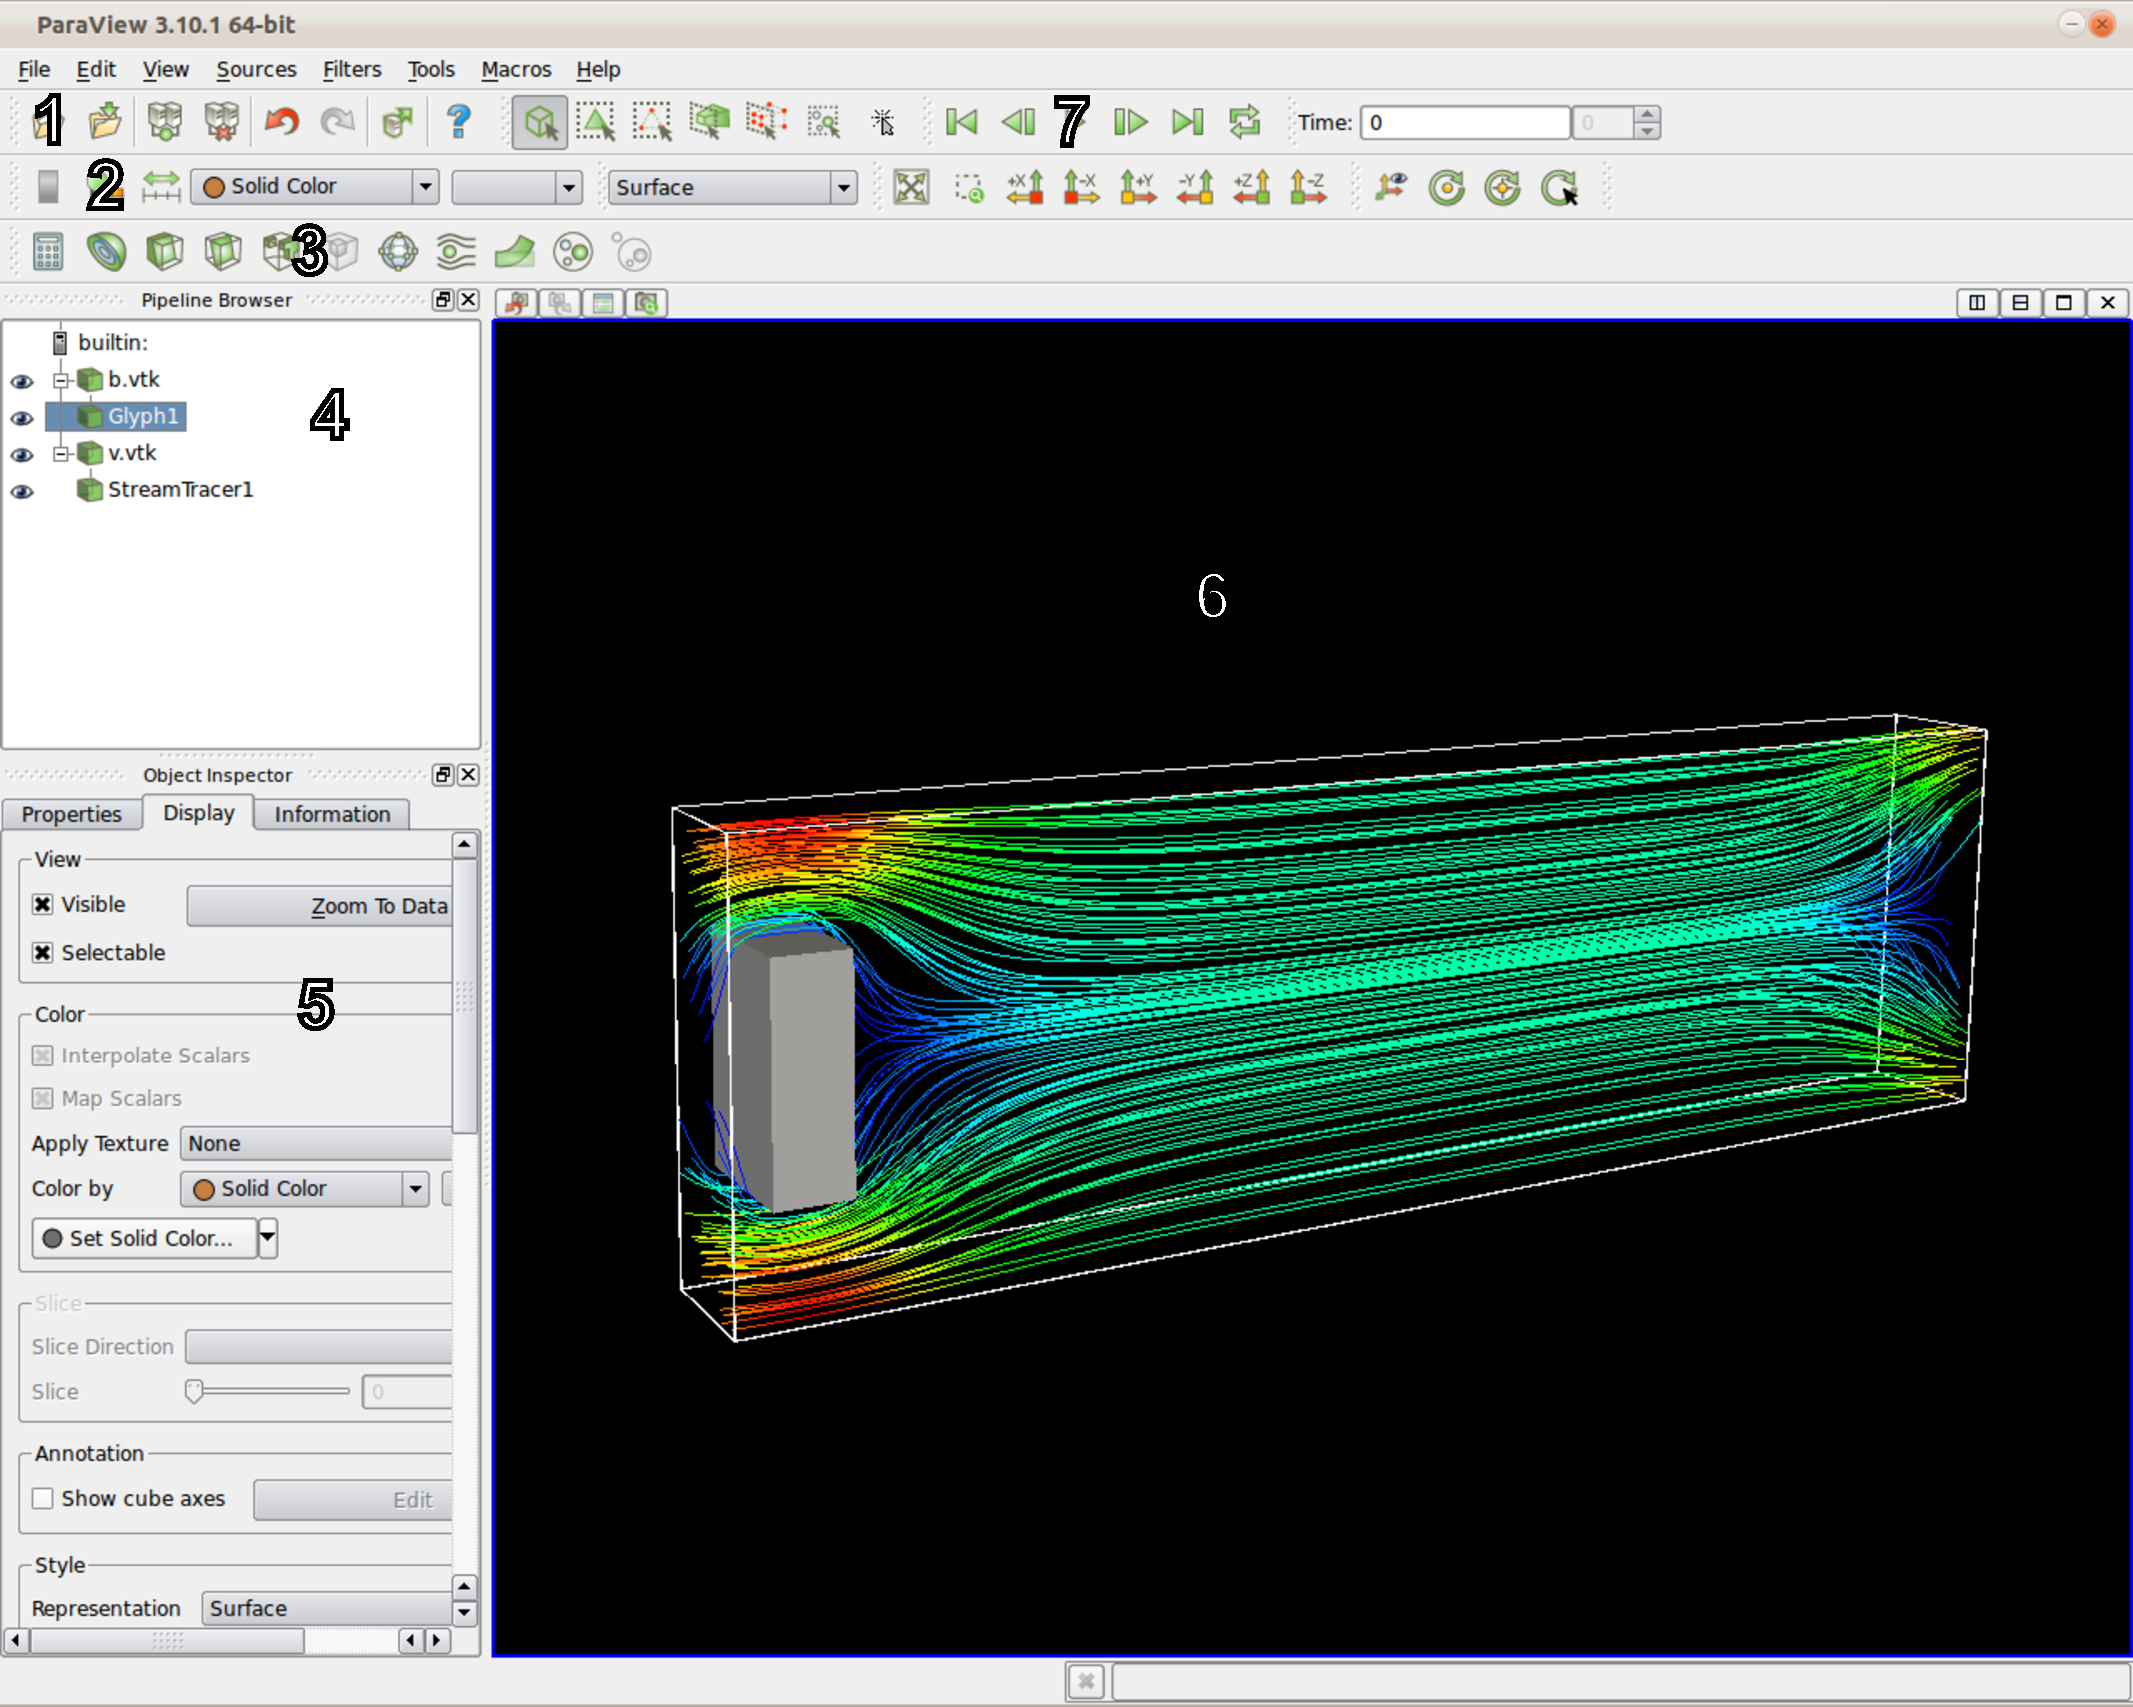
\includegraphics[width=1.0\textwidth]{figures/paraview.pdf}
  \caption{Paraview with a sample visualization and the most important controls.}
  \label{fig:paraview}
\end{center}
\end{figure}
%
\begin{enumerate}
\item Load data files into the pipeline for visualization
\item Adjust color settings of the filter selected in the pipeline browser
\item Add one of the most used filters to the element selected in the pipeline browser
\item The pipeline browser -- shows loaded data files and filter applied to them for visualization
\item Configuration panel for the filter chosen in the pipeline browser
\item The preview panel -- you can rotate, zoom and move this with the mouse
\item Controls for videos
\end{enumerate}
%
For a start it makes sense to use a \textit{Glyph} filter to visualize particle positions and a \textit{Slice}, \textit{Streamline}, or \textit{Glyph} filter for LB velocity fields. With a little exploration, these controls should be self explanatory. If you need help, don't hesitate to consult your tutor, the Paraview help (F1) or the Paraview online documentation at \href{http://www.paraview.org}{http://www.paraview.org}.

\pagebreak
